%\chapter{det-overview}

%%%%%%%%%%%%%%%%%%%%%%%%%%%%%%%%%%%%%%%%%%%%%%
\section{Detector Requirements}

insert detector overview here

%%%%%%%%%%%%%%%%%%%%%%%%%%%%%%%%%%%%%%%%%%%%%%
\section{Liquid argon detector properties}
- Electron drift + LAr purity etc.
- LAr scintillation light 

%%%%%%%%%%%%%%%%%%%%%%%%%%%%%%%%%%%%%%%%%%%%%%
\section{TPC Signal Formation (Xin)}

The principle of the large single-phase LArTPC with wire readouts is shown in 
Fig.~\ref{fig:signal}. When charged particles traverse through the LAr medium,
ionization electrons are generated. They would travel at a constant speed 
($\sim$1.6 km/s at 500 V/cm electric field) along the external electric field 
toward the multiple anode wire planes. The first wire planes encountered collect 
an induction signals as the drifting charge passes through.  The charge is collected 
on the wires in the final plane. This transparency of the induction planes is assured by 
by applying an appropriate bias voltage to these wire planes.
During this process, current will be produced on the wire planes. 
Since the locations of wires are accurately known, the position of the
ionization charge in the direction transverse to the drift can be determined in 
three independent views. The time of the initial interaction is determined by collecting 
scintillation light 
in a fast optical detector system.
Measuring the time from this prompt activity to signals on the wires it is 
possible to determine the longitudinal position along the drift direction.
Therefore, one can achieve a 3D imaging of the trajectories of the charged particles in the LAr. 
The amount of ionization electrons depends on the energy and type of
the initial particles, and can be used to deduce their properties.

\begin{figure}[htb]
\centering
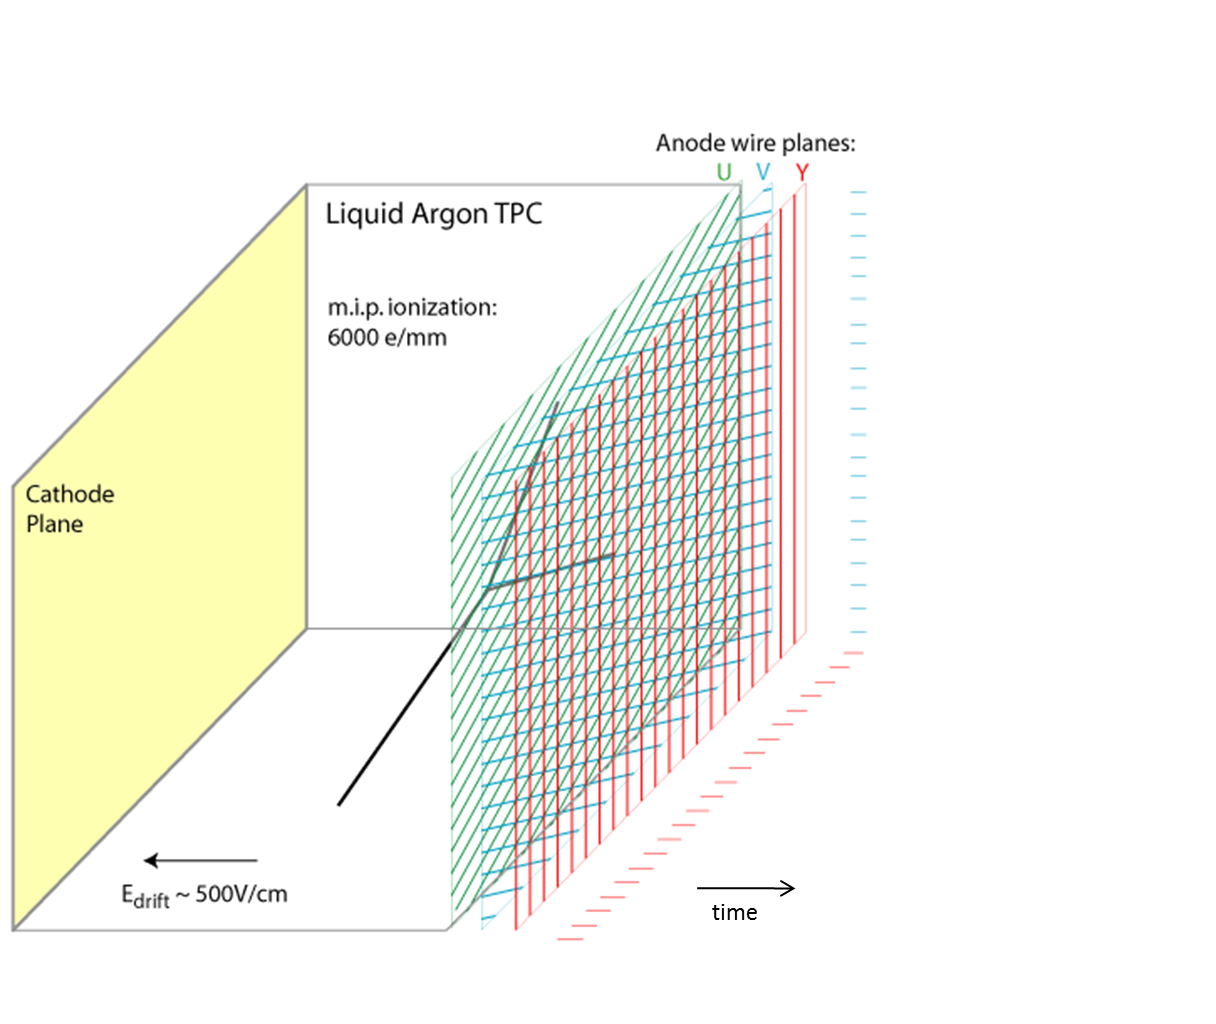
\includegraphics[width=0.48\textwidth]{figures/TPC_1.png}
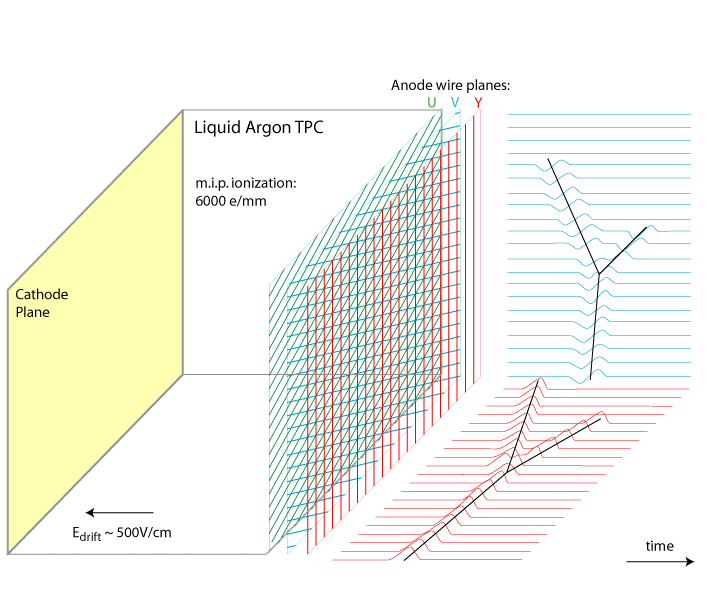
\includegraphics[width=0.48\textwidth]{figures/TPC_2.png}
\caption{The principles of LArTPC are shown. (left) When energetic, charged particles 
traverse the LAr medium, ionization electrons are produced and move
along the external electric field towards the anode planes. (right) The ionization
electrons pass through the induction wire planes and are  collected by the 
final collection wire plane. 
During this process, signals are measured on the wires
in each plane which provides information about the 3D positions and
energies of initial particles.}
\label{fig:signal}
\end{figure}


%%%%%%%%%%%%%%%%%%%%%%%%%%%%%%%%%%%%%%%%%%%%%%
\section{Space charge effects}

%%%%%%%%%%%%%%%%%%%%%%%%%%%%%%%%%%%%%%%%%%%%%%
\section{...}
